\documentclass[a4paper, twoside, openright]{article}
\usepackage[T1]{fontenc}
\usepackage[utf8]{inputenc}
\usepackage[english,italian]{babel}
\usepackage{graphicx}
\usepackage{lipsum}
\usepackage[a4paper,top=3cm,bottom=3cm,left=3cm,right=3cm]{geometry}
\usepackage[fontsize=12pt]{scrextend}
\raggedbottom
\linespread{1.25}
\usepackage{fancyhdr}
\usepackage{amsmath}
\usepackage{hyperref}

\usepackage{xcolor}
\usepackage{listings}
\usepackage{caption}

% Definisci i colori che desideri utilizzare
\definecolor{codebackground}{rgb}{0.95,0.95,0.95}
\definecolor{codeframe}{rgb}{0.75,0.75,0.75}
\definecolor{codekeyword}{rgb}{0.37,0.08,0.25}

% Impostazioni per il blocco di codice
\lstset{
    language=Python,
    basicstyle=\ttfamily\small,
    keywordstyle=\color{codekeyword}\bfseries,
    backgroundcolor=\color{codebackground},
    frame=single,
    rulecolor=\color{codeframe},
    breaklines=true,
    showstringspaces=false,
    captionpos=b,
}


\pagestyle{fancy}
\fancypagestyle{plain}{%
  \renewcommand{\headrulewidth}{15pt}%
  \fancyhf{}%
}

\usepackage{subfig}
\usepackage{float}
\graphicspath{ {./images/} }

\definecolor{linkColor}{RGB}{2,11,120}
\definecolor{printLinkColor}{RGB}{0,0,0}

\usepackage[colorlinks=true, allcolors=printLinkColor]{hyperref}
\newcommand\anchor[2]{%
  \href{#2}{#1}\footnote{\url{#2}}%
}

\usepackage{tgschola}

\definecolor{bgTitleRed}{RGB}{85,45,50}
\fancyhf{}
\fancyfoot[R]{\thepage}


\begin{document}

%caption dei listings è in bold
\captionsetup[lstlisting]{labelfont={bf}}

\begin{figure}[H]
    \centering
    
\includegraphics[width=7cm]{img/logo.png}
\end{figure}

\begin{center}
    \LARGE{UNIVERSITÀ DI SALERNO}
    \vspace{1mm}
    \\ \large{DIPARTIMENTO DI INFORMATICA }
    \vspace{5mm}
\end{center}

% Titolo e
\vspace{10mm}
\begin{center}
    {\LARGE{\bf \textit{MetaClassAI}\\\vspace{5mm} Regressore per la stima della durata ideale dei meeting}}
\end{center}

\vspace{5mm}
\begin{center}
    \centering
    \large{Repository GitHub:}
    \href{https://github.com/smike18181/MetaClass_FIA}{\textcolor{blue}{https://github.com/smike18181/MetaClass\_FIA}}
\end{center}

\vspace{20mm}

% Definzione autori
\begin{center}
        {\centering
        \large {Compilato da:} \\
        \vspace{2mm}
        \normalsize \textbf{Pesce Michele} \\
        \vspace{2mm}
        \normalsize \textbf{Alberti Salvatore} \\
        \vspace{2mm}
        \normalsize \textbf{Gatto Francesco} \\
        \vspace{2mm}
        \normalsize \textbf{Cavaliere Domenico} \\}   
\end{center}    

% Index page
\newpage
\fancyhead[R]{ Indice } %RO=right odd, LE=left even
\tableofcontents

% Footer setting
\newpage
\fancyfoot[R]{\thepage}

% Chapters
\section{Definizione del problema}
\fancyhead{}    % reset header
\fancyhead[RO,LE]{Definizio del problema}

\subsection{Obiettivi}
\fancyhead{}    % reset header
\fancyhead[RO,LE]{Obiettivi}
\subsection{Specifica PEAS}
\fancyhead{}    % reset header
\fancyhead[R]{Specifica PEAS}
\par{
\begin{itemize}
    \item \textbf{Performance}: La misura di performance dell'agente è la precisione con cui si avvicina alla reale durata media del meeting quando questa viene proposta in fase di programmazione;
    \item \textbf{Environment}: L'ambiente in cui opera l'agente è l'insieme dei feedback degli utenti a fine meeting del nostro applicativo;
    \item \textbf{Actuators}:Gli attuatori a disposizione dell'agente sono le caselle di input del range orario, che presenta già l'offset basato sulla stima fatta sulla fascia oraria proposta quando si va a schedulare un meeting sul sito \url{https://metaclass.commigo.it};
    \item \textbf{Sensors}: I sensori tramite il quale l'agente recepisce stimoli dall'ambiente sono i report compilabili sul sito \url{https://metaclass.commigo.it} e sul tempo di utilizzo del visore per singolo utente all'interno di un meeting;
\end{itemize}
}

\subsubsection{Caratteristche dell'ambiente}
\fancyhead{}    % reset header
\fancyhead[R]{Caratteristche dell'ambiente}
\subsection{Analisi del problema}
\fancyhead{}    % reset header
\fancyhead[R]{Analisi del problema}
\par{
Una soluzione al problema inerente sarebbe potuta essere sviluppata mediante una semplice media della durata di tutti i meeting svolti dagli utenti, tuttavia tale soluzione avrebbe comportato diverse limitazioni:
\begin{itemize}
    \item questa implementazione non tiene conto di caratteristiche specifiche dell'utente, come ad esempio una fascia d'età più bassa che può essere maggiormente predisposta ad una durata più lunga di utilizzo del visore;
    \item non ci sarebbe stato un accesso immediato ad una quantità di dati adeguata;
    \item l'output risultante potrebbe risultare impreciso, non avendo l'operazione definita una quantità di dati eterogenei sufficientemente grande per fornire un risultato attendibie;
\end{itemize}
Date queste limitazioni, si èdeciso di affrontare il problema in esame adottando tecniche di Machine Learning in grado di effettuare la \textbf{user segmentation}, andando cioè a suddividere gli utenti in gruppi distinti in base a caratteristiche condivise (e.g. sesso, età, motion sickness level).\\
Sono stati presi in analisi diversi algoritmi di Machine Learning, la cui scelta è infine ricaduta su di un problema di regressione lineare multipla.\\
Idea di base è quella di raccogliere i report inseriti da ogni utente all'interno del sistema, unitamente alla durata del meeting per singolo utente che viene presa direttamente tramite l'applicativo VR, e dati relativi a sesso ed età per singolo utente automaticamente dal sistema stesso, il tutto viene fatto al termine di ogni meeting.\\
Sulla base di questi dati raccolti verrà poi fatta la predizione della durata consigliata per il meeting in fase di scheduling.
}

\begin{document}
\end{document}
\newpage
\section{Dataset}
\fancyhead[]{}
\fancyhead[R]{ Dataset }

\subsection{Scelta del dataset}
\fancyhead{}    % reset header
\fancyhead[R]{Scelta del dataset}
\par{
L'acquisizione dei dati rappresenta il primo fondamentale passo nel processo di sviluppo di un modello di intelligenza artificiale. Questo processo consiste nella raccolta, nell'organizzazione e nella preparazione dei dati necessari per addestrare e valutare il modello.\newline
Dopo un'accurata fase di ricerca, si è proceduto con la creazione del dataset necessario per il modello di intelligenza artificiale finalizzato alla stima della durata consigliata per l'utilizzo dell'esperienza VR.\newline
Tale dataset è stato ottenuto tramite la \textbf{modellazione} e \textbf {l'elaborazione} di dati preesistenti, i quali sono stati ricavati dal sito \href{https://www.kaggle.com/}{\textbf{kaggle.com}}.\newline
In particolare, il dataset scelto è stato il seguente: \href{https://www.kaggle.com/datasets/aakashjoshi123/virtual-reality-experiences/data}{\textbf{Virtual Reality Experiences}}.\newline
Questo dataset, reso disponibile con licenza pubblica, consiste in un insieme di \textbf{1000 istanze} ricavate dalle esperienze di  utenti all'interno di ambienti di realtà virtuale (VR),
comprendendo informazioni sulle risposte fisiologiche e emotive degli utilizzatori del sistema.
}
\subsection{Analisi Dataset e ei dati al suo interno}
\fancyhead{}    % reset header
\fancyhead[R]{Analisi Dataset e ei dati al suo interno}
\par{
Le fonti del dataset sono costituite principalmente da informazioni ricavate da studi effettuati in laboratorio.
\textbf{il Dataset si compone delle seguenti sette caratteristiche:}\newline
\begin{itemize}
  \item Primo elemento
  \item Secondo elemento
  \item Terzo elemento
\end{itemize}
}
\subsection{Incremento del dataset}
\fancyhead{}    % reset header
\fancyhead[R]{Incremento del dataset}

\newpage
\section{ Ingegnerizzazione dei dati }
\fancyhead[]{}
\fancyhead[R]{ Ingegnerizzazione dei dati }

\subsection{Data cleaning}
\fancyhead{}    % reset header
\fancyhead[R]{Data cleaning}
\label{paragrafo 3.1}
Nella prima fase di ingegnerizzazione dei dati ci siamo soffermati sul data cleaning, ovvero siamo andati ad analizzare i dati valutando se ci fossero valori nulli o non validi.
Da un analisi preliminare dei dati a nostra disposizione è risultato che:

\begin{figure}[h]
    \centering
    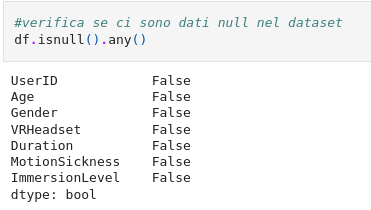
\includegraphics[width=0.75\textwidth]{MetaClassAI_Documentazione/3/img/ValoriNULLDataset.png}
    \caption{Esempio di verifica dei dati per valori nulli}
    \label{fig:verifica-null-dataset}
\end{figure}

\begin{figure}[h]
    \centering
    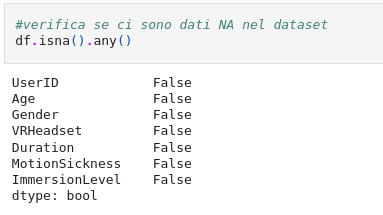
\includegraphics[width=0.75\textwidth]{MetaClassAI_Documentazione/3/img/ValoriNADataset.png}
    \caption{Esempio di verifica dei dati per valori N/A}
    \label{fig:verifica-NA-dataset}
\end{figure}
Come si può notare, non sono presenti dati nulli o invalidi tra quelli presenti, per cui non sono state necessarie tecniche di Data cleaning.

\subsection{Feature scaling}
\fancyhead{}    % reset header
\fancyhead[R]{Feature scaling}
\newpage
\subsection{Feature selection}
Nella terza fase ci siamo focalizzati sulla feature selection con l’obiettivo di definire delle caratteristiche, anche chiamate feature, metriche, o variabili indipendenti che possano caratterizzare gli aspetti principali del nostro problema in esame e, quindi, avere una buona potenza predittiva. Abbiamo utilizzato un metodo della libreria \textit{matplotlib}, il quale ci ha permesso di visualizzare le dipendenze tra le diverse variabili.

\begin{figure}[h]
    \centering
    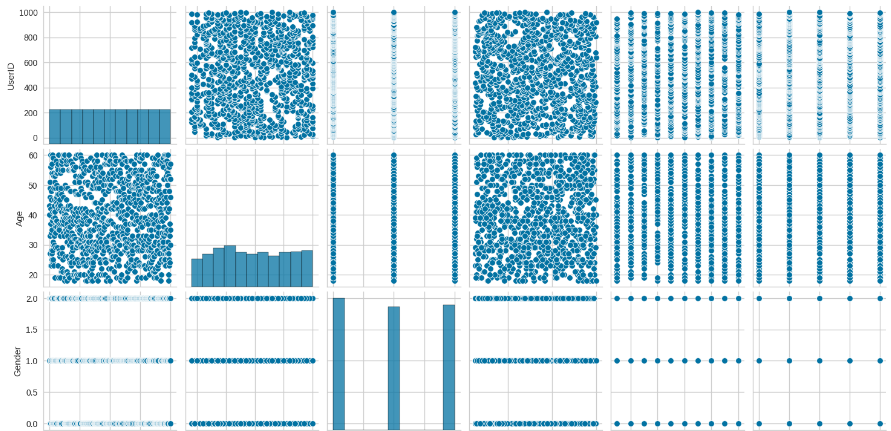
\includegraphics[width=\textwidth]{MetaClassAI_Documentazione/3/img/FeatureSelection_1.png}
\end{figure}
\begin{figure}[h]
    \centering
    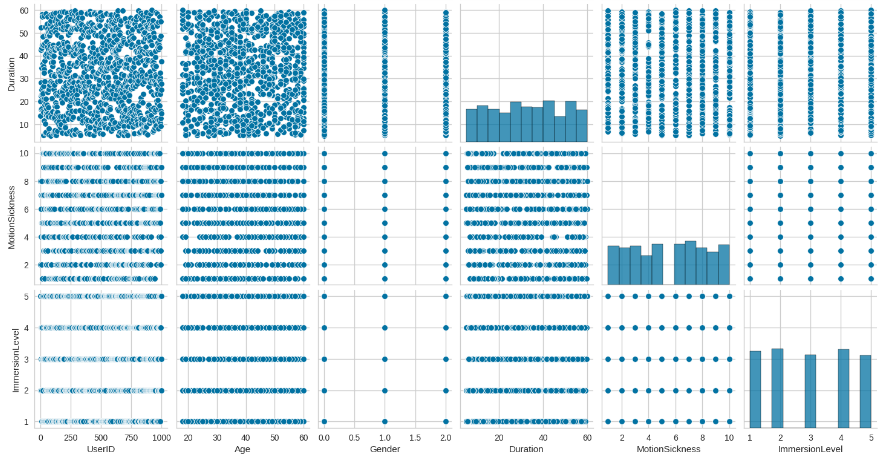
\includegraphics[width=\textwidth]{MetaClassAI_Documentazione/3/img/FeatureSelection_2.png}
\end{figure}
\newpage
\subsection{Data Balancing}

Nella quarta fase ci siamo focalizzati sul Data balancing, ovvero un insieme di tecniche per convertire un dataset sbilanciato in un dataset bilanciato. Nel nostro caso, trattandosi di un problema di regressione lineare multipla, non abbiamo avuto la necessità di verificare il bilanciamento delle classi, poiché abbiamo dati dal valore continuo.




\newpage
\section{ \textbf{Soluzione}\textbf{ al problema} }
\fancyhead[]{}
\fancyhead[R]{Ingegnerizzazione dei dati }

\subsection{Model evaluation}
\fancyhead{}    % reset header
\fancyhead[R]{Model evaluation}

In seguito alla definizione delle tecniche di ingegnerizzazione dei dati dell’agente intelligente, è necessario stabilire le \textbf{metriche} e le \textbf{tecniche} di validazione delle prestazioni dello
stesso. Occorre suddividere l’insieme dei dati fin’ora analizzato in due insiemi: 
\begin{itemize}
\item \textbf{training set}:
composto dalle istanze di dati che saranno utilizzate per l’addestramento.
\item \textbf{test set}, composto dalle istanze di dati per cui l’agente dovrà predire il valore della variabile dipendente.
\end{itemize}
Abbiamo preso in considerazione diverse tecniche per effettuare questa suddivisione: \textit{K-Fold
validation, Stratified K-fold validation, Repeated K-fold validation e Repeated Stratified
K-fold validation}. In particolare, le tecniche \textit{Stratified K-fold} e \textit{Repeated Stratified} sono state
scartate in quanto non risultano adatte ad essere applicate su dati continui e a dataset con più
variabili indipendenti. \\ 
Per tutte è stato necessario definire il valore di K, ovvero il numero
di gruppi utilizzati per suddividere il dataset in test e training set, mentre per le tecniche di tipo "Repeated" è stato stabilito anche il numero di
ripetizioni di validazione da effettuare. Le metriche che sono state impiegate per valutare la bontà delle
previsioni effettuate sono state:
\subsection{Regressione}
\fancyhead{}    % reset header
\fancyhead[R]{Regressione}
\subsubsection{Regressione lineare}
\fancyhead{}    % reset header
\fancyhead[R]{Regressione lineare}
Una volta definito il processo di feature engineering e scelte le tecniche di valutazione, è
stato possibile definire un modello di regressione lineare tramite la libreria \textit{sklearn.linearmodel},
in particolare si è utilizzato il metodo \textit{fit} per addestrare il modello sull’insieme dei dati di
training e in seguito \textit{predict} sull’insieme dei dati di test per predirne il valore della variabile
dipendente basandoci sulle feature dell’insieme di dati di training.
Prima di procedere con la creazione del modello di regressione lineare multipla, abbiamo
verificato che i nostri dati rispettassero le condizioni di:
\par{
\begin{itemize}
    \item \textbf{Linearità dei dati}
    \begin{figure}[H]
        \centering
        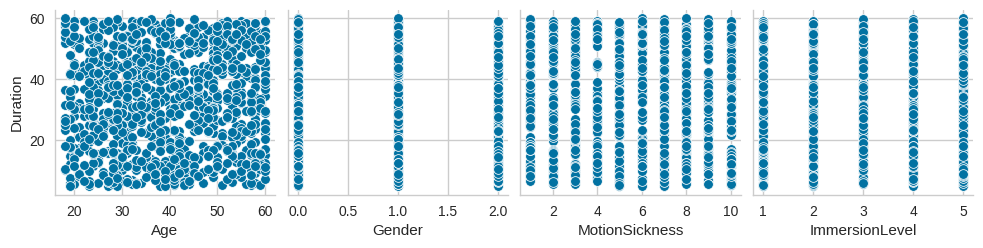
\includegraphics[width=1\linewidth]{image.png}
        \caption{Linearità dei dati}
        \label{fig:enter-label}
    \end{figure}
    da come si nota in figura, si hanno dei dati che hanno una distribuzione omogenea e lineare rispetto alla variabile dipendente \textit{Duration}.
    \item \textbf{Bassa multicollinearità}
    \begin{figure}[H]
        \centering
        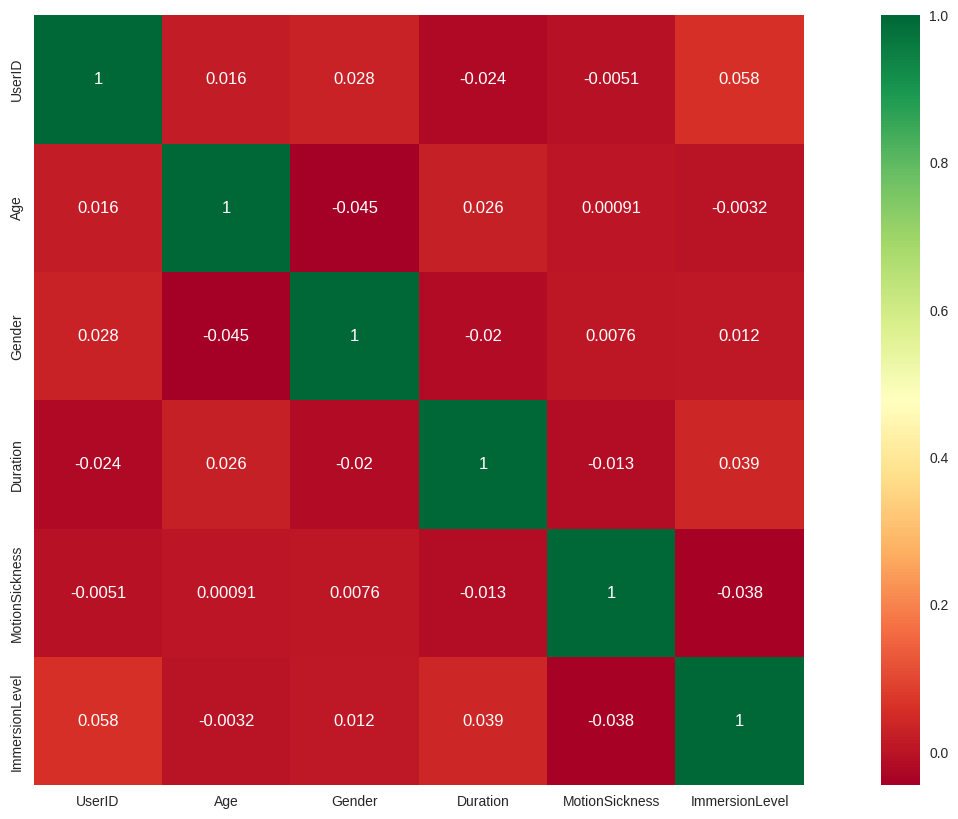
\includegraphics[width=1\linewidth]{multicoll.png}
        \caption{Multicollinearità}
        \label{fig:enter-label}
    \end{figure}
    in quest'altra figura invece si nota che le feature utilizzate nel dataset non sono fortemente correlate tra loro, quindi consente al modello di applicare una regressione lineare multipla senza preoccuparsi di avere variabili ridondanti durante l'addestramento.
\end{itemize}
}

Al fine di definire il modello che si adatti meglio i dati, è stato necessario applicare il \textbf{metodo empirico}, cioè l'utilizzo di vari algoritmi di regressione al fine di trovare quello più adatto al problema in esame.\\
Per ogni modello creato, sono stati applicate 3 diverse tipologie di normalizzazione del dataset per poter scegliere in modo più accurato il modello da utilizzare. Le 3 normalizzazioni sono:
\par{
\begin{itemize}
    \item \textbf{Z-Score normalization}\\
    \begin{equation}
        Z = \frac{x - \mu}{\sigma}
    \end{equation}
    \item \textbf{MinMax normalization}
    \begin{equation}
        X_{\text{norm}} = \frac{X - X_{\text{min}}}{X_{\text{max}} - X_{\text{min}}}
    \end{equation}
    \item \textbf{Robust scaling}
    \begin{equation}
        X_{\text{robust}} = \frac{X - \text{Mediana}}{\text{IQR}}
    \end{equation}
\end{itemize}
}\\

Infine, oltre alle 3 metriche descritte nel paragrafo \ref{paragrafo 4.1}, per poter valutare la validità delle stime è stato fatto un controllo e un plot dei \textbf{residui} ricavati durante l'esecuzione del modello sul \textit{test set}. \\
Più in dettaglio abbiamo verificato:
\par{
\begin{itemize}
    \item \textbf{normalità dei residui}: se i residui vengono \textbf{normalmente distribuiti} cioè se i residui seguono o meno una distribuzione approssimativamente normale. Si guarda se la forma della distribuzione è a campana simmetrica.
    \item \textbf{omoschedasticità}: se gli errori residui hanno una varianza \textbf{costante}, cioè commettono un tasso di errore costante.
    \begin{figure}[H]
        \centering
        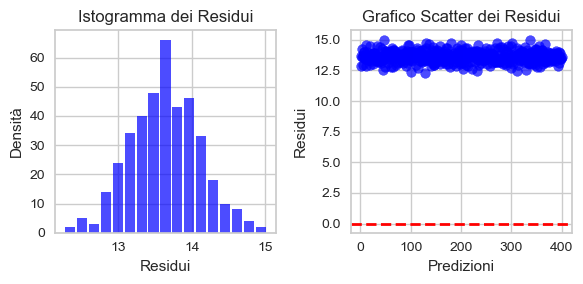
\includegraphics[width=1\linewidth]{plotresidui.png}
        \caption{Esempio di plot dei residui}
        \label{fig:enter-label}
    \end{figure}
\end{itemize}
}

Partendo dalle metriche è stata deinita una semplice classe che contesse 3 array di tutte le metriche ricavate durante la fase di validazione: \\
\begin{lstlisting}[caption=Classe Metrics1]
#oggetto che contiene le metriche
class Metrics1:
  #costruttore
  def __init__(self,mae,mse,rmse):
    self.mae=mae      #MAE
    self.mse=mse      #MSE
    self.rmse=rmse    #RMSE

  #ToString
  def __str__(self):
    return f'Metrics [mae= {self.mae} mse= {self.mse} rmse= {self.rmse} mean= {np.mean([self.mae,self.mse,self.rmse])}'
\end{lstlisting} 

Tale classe è servita definire MetricsResultContainer, un ulteriore classe che funge da "ambiente" per poter eseguire metodi specifici sul plot dei residui e sulla stampa delle metriche in base al modello e alla tipologia di normalizzazione utilizzata: \\
\begin{lstlisting}[caption=MetricsResultContainer]

class MetricsResultContainer:
    meanMAE = []
    meanMSE = []
    meanRMSE = []

    def __init__(self, model, alg, scaler, param, metricsMean):
        self.model = model
        self.alg = alg
        self.scaler = scaler
        self.param = param
        self.metricsMean = metricsMean
        self.meanMAE = []
        self.meanMSE = []
        self.meanRMSE = []
        

    def printMetrics(self):
        for m in self.metricsMean:
            self.meanMAE.append(m.mae)
            self.meanMSE.append(m.mse)
            self.meanRMSE.append(m.rmse)
        print("meanMAE=", np.mean(self.meanMAE))
        print("meanMSE=", np.mean(self.meanMSE))
        print("meanRMSE=", np.mean(self.meanRMSE))
        
        self.visualizza_grafici()
        self.test_Durbin_Watson()

    # funzione per mostrare la normalità dei residui e l'omoschedasticità
    def visualizza_grafici(self):
        fig, axs = plt.subplots(1, 2, figsize=(6, 3))  # Una riga, due colonne

        # Istogramma dei Residui
        axs[0].hist(self.meanMAE, bins='auto', color='blue', alpha=0.7, rwidth=0.85)
        axs[0].set_title('Istogramma dei Residui')
        axs[0].set_xlabel('Residui')
        axs[0].set_ylabel('Densità')

        # Grafico Scatter dei Residui
        lunghezza_dati = len(self.meanMAE)
        axs[1].scatter(np.arange(1, lunghezza_dati + 1), self.meanMAE, color='blue', alpha=0.7)
        axs[1].axhline(y=0, color='red', linestyle='--', linewidth=2)
        axs[1].set_title('Grafico Scatter dei Residui')
        axs[1].set_xlabel('Predizioni')
        axs[1].set_ylabel('Residui')

        plt.tight_layout()  # Assicura una corretta disposizione dei grafici senza sovrapposizioni
        plt.show()
\end{lstlisting}
Nel costruttore è stato inserita anche la tecnica di convalida utilizzata (denominata come model). In questa fase ne sono state decise 2 in particolare:
\par{
\begin{itemize}
    \item \textbf{K-fold cross validation}: metodo statistico che consiste nella ripetuta partizione e valutazione dell’insieme dei dati di partenza. 
    \item \textbf{Repeated K-fold validation}: Si ripete N volte la K-fold cross validation.
\end{itemize}
}
Prima di fare ciò era necessario comprendere il numero adatto di partizioni da avere nel dataset utilizzando la formula:
\begin{equation}
    k= (len(df)/(len(df)*0.3))
\end{equation}
dove len(df) indica il numero di campioni del nostro dataset. Il K così ottenuto è uguale a 3.
\subsection{Algoritmi}
\fancyhead{}    % reset header
\fancyhead[R]{Algoritmi}
\label{paragrafo 4.3}

Prima di parlare degli algoritmi è necessario trattare come viene effettuata la generazione del modulo.
Il tutto viene fatta da una funzione chiamata \textit{generateModel()}:\\

\begin{lstlisting}
   #funzione per generare il modello, divisione training e test, features scaling, selection
   def generateModel(alg, scaler, model, select)
\end{lstlisting}



\par{
\begin{itemize}
    \item \textbf{alg}: metodo di convalida utilizzato nella validazione del modello
    \item \textbf{scaler}: tecnica di normalizzazione dei dati usata
    \item \textbf{model}: algoritmo di regressione
    \item \textbf{select}: insieme delle feature selezionate 
\end{itemize}
}

L'obiettivo del metodo è quello di effettuare la divisione del dataset in test e training set per poi eseguire per poi applicare operazioni di data engeening per preparare i dati. \\
\begin{lstlisting}
    # suddivisione in training e test test
    X_train, X_test = X.iloc[train_index], X.iloc[test_index]
    y_train, y_test = y.iloc[train_index], y.iloc[test_index]
    #feature scaling sui traing test
    X_train_z = scaler.fit_transform(X_train)
    X_test_z = scaler.transform(X_test)
    #applicazione feature selection su train_z
    X_train_z = select.fit_transform(X_train_z, y_train)
    X_test_z = select.transform(X_test_z)
\end{lstlisting}
La suddivisione avviene andando a scegliere il numero di partizioni k per poi applicare l'algoritmo di suddivisione del dataset.\\
\begin{lstlisting}
    #numero record nel dataset
    k=len(df)
    #calcolo k ideale da usare nelle tecniche di validazione deve essere il 30% della lunghezza del dataset
    k= (k/(k*0.3))
   #Kf divisione dataset per k gruppi per testare mediante due algoritmi Kfold-RepeateKFold
   kf = KFold(n_splits=int(np.ceil(k)),random_state=42, shuffle=True)
   #rKf con k gruppi, e 10 ripetizioni
   rkf = RepeatedKFold(n_splits=int(np.ceil(k)), n_repeats=100, random_state=42)
\end{lstlisting}

Da come si vede dal codice, vengono applicati i metodi descritti nel paragrafo \ref{paragrafo 4.2.1}. \\
A questo punto l'unica cosa da fare è l'addestramento è la validazione:
\begin{lstlisting}
     #training dell'algoritmo sui 
     training set
    clone_model.fit(X_train_z,y_train)
    #validazione modello e applicazione predizione sui testSet
    y_pred = clone_model.predict(X_test_z)
\end{lstlisting}
Questo blocco è rinchiuso in un \textit{for}, quindi il valore predetto \textit{ypred} è unico. \\
Col valore presetto si ricavano i \textbf{residui} descritti nel paragrafo \ref{paragrafo 4.2.1} andando poi a ricavare le 3 metriche di valutazione dei modelli.

\begin{lstlisting}
     metrics1.append(
        Metrics1(metrics.mean_absolute_error(y_test,y_pred),
                 metrics.mean_squared_error(y_test,y_pred),
                 np.sqrt(metrics.mean_squared_error(y_test,y_pred))
                 )
        )
  return metrics1
\end{lstlisting}
metrics è un'istanza della classe \textit{MetricsResultContainer} che consente di poter stampare le metriche e visualizzare i grafici in caso di utilizzo di regressione lineare. \\
\subsubsection{Algoritmo scelto}
\fancyhead{}    % reset header
\fancyhead[R]{Algoritmo scelto}
\subsection{Creazione modello finale}
\fancyhead{}    % reset header
\fancyhead[R]{Creazione modello finale}



\newpage
\section{ Inteazione con MetaClass }
\fancyhead[]{}
\fancyhead[R]{ Interazione con MetaClass }

\subsection{Stima durata dei meeting}
\fancyhead{}    % reset header
\fancyhead[R]{Stima durata dei meeting}
\label{paragrafo 5.1}
\subsection{Aggiunta istanze}
\fancyhead{}    % reset header
\fancyhead[R]{Aggiunta istanze}
\label{paragrafo 5.2}

MetaClass,come descritto prima, consente la compilazione di un questionario, dopo un meeting a cui ha partecipato l'utente, è terminato.
I dati del questionario vengono presi per incrementare il dataset, infatti oltre al motionSickenss e al Immersivity Level, si prelevano dati come età e sesso.
Per poter inserire la tupla nel dataset ci occorre però un modo per poter ricavare lo \textit{UserID} dell'ultima istanza del dataset per incrementarla e farla diventare lo \textit{UserID} della prossima tupla da inserire.
Per fare ciò è stato necessario utilizzare la libreria \textit{org.apache.commons} per poter fare la lettura e la scrittura in un file formato csv (formato di estrazione del dataset). \\
\begin{lstlisting}
import org.apache.commons.csv.CSVFormat;
import org.apache.commons.csv.CSVParser;
import org.apache.commons.csv.CSVPrinter;
import org.apache.commons.csv.CSVRecord;
\end{lstlisting}
Questi sono gli oggetti utilizzati per accedere a un file csv, in particolare:
\par{
\begin{itemize}
    \item \textbf{CSVFormat}:
     Questo oggetto definisce il formato del file CSV, specificando opzioni come il separatore di colonne, il carattere di escape e altri parametri di formattazione. Viene utilizzato per configurare la lettura e la scrittura dei file CSV.
     \item \textbf{CSVParser}:
     Questo oggetto è responsabile della lettura di un file CSV, analizzandolo e convertendo i dati in oggetti di tipo CSVRecord. Utilizza il CSVFormat per interpretare correttamente la struttura del file CSV.
     \item \textbf{CSVPrinter}:
      Questo oggetto viene utilizzato per la scrittura di dati in un file CSV. Accetta dati in forma di oggetti CSVRecord e li formatta secondo il CSVFormat specificato, scrivendoli nel file CSV di output.
      \item \textbf{CSVRecord}:
      Rappresenta una singola riga di dati in un file CSV. I valori dei singoli campi sono accessibili attraverso metodi come get o tramite l'indicizzazione. Viene utilizzato sia durante la lettura dei file CSV da CSVParser che durante la scrittura da CSVPrinter.
\end{itemize}
}

Ottenuta la tupla risultante, è possibile inserirla nel dataset: \\

\begin{lstlisting}
    // Aggiunta della nuova tupla di valori al CSV
        csvPrinter.printRecord(
            ultimoUserId + 1, // UserID
            periodo.getYears(), // Age
                (u.getSesso().equals("M") ? 2 : (u.getSesso().equals("F")  ? 1 : 0)), // Gender
            null, // VR Headset (non utilizzato e rimosso nella feature selection)
            (double) durata.toMinutes(), // Duration
            immersionLevel, // ImmersionLevel
            motionSickness); // MotionSickness
\end{lstlisting}

Da come si può notare il sesso è stato espresso come un valore numerico (per consentire lo scaling durante il training del modello) e la cella relativa all'headSet è nulla in quanto verrà eliminata a prescindere durante le feature selection. \\
Infine una questione importante ce l'ha l'attributo Duration che è stato ricavato andando a fare una media di tutti i minuti in cui è stato l'utente all'interno dei meetings (considerando però anche le altre stanze in cui ha accesso).  

Infine dopo l'inserimento di dati era necessario stabilire quando effetturare il \textbf{retraining del modello} avendo a disposizione 2 alternative:
\par{
\begin{itemize}
   \item \textbf{allenarlo dopo ogni utente aggiunto}
   \item \textbf{allenarlo dopo n inserimenti}
\end{itemize}
}
A primo impatto sembra che la prima opzione sia la migliore, in quanto si ha fin da subito il modello riallenato e quindi fornire stime fin da subito più accurate, ma questo porta come svantaggio un esecuzione lenta nella compilazione del questionario. In parole povere, quando l'utente compila un questionario, dovrà attendere diversi secondi per avere un feedback di avvenuta compilazione, rendendo quindi il sistema meno usabile.
A valle di ciò si è deciso di implentare la seconda opzione, dove \textbf{ad ogni 100 inserimenti} veniva inserita effettuato il retraining:
\begin{lstlisting}
     //incremento il contatore che mi tiene traccia di quante tuple vengono aggiunte
        counter++;
      //ogni 100 inserimenti avviene il retraining
      if ((counter% 100) == 0) {
        // ri-training del modello
        trainingModel();
      }
\end{lstlisting}
Per fare ciò è servito un contatore statico che veniva incrementato ad ogni inserimento, poi in un if veniva controllato se il contatore ha un modulo pari a 100 (cioè se sono stati inserite 100 tuple).


\subsection{Retraining del modello}
\fancyhead{}    % reset header
\fancyhead[R]{Retraining del modello}

Una volta inserite le nuove istanze al termine della compilazione del questionario, il modello deve essere \textbf{riallenato} considerando i nuovi valori inseriti.\vspace{1ex}
Per fare ciò è stato necessario creare un \textbf{modulo python} che contenesse un \textbf{interprete} e \textbf{un'ambiente virtuale} in grado di installare tutte le liberie necessarie per l'esecuzione di un file python \textcolor{gray!50!black}{\textit{(trainingModel.py)}} contenente il codice necessario per fare ciò. \\ 

\begin{lstlisting}[caption=Prelievo del dataset]
    # coding: utf-8
    import pandas as pd
    
    FILE_NAME = "../src/main/resources/ModuloAI/data.csv"
    
    # Verifica il contenuto del file
    try:
        df = pd.read_csv(FILE_NAME)
    except pd.errors.EmptyDataError:
        print("Il file CSV e' vuoto.")
    except pd.errors.ParserError:
        print("Errore di parsing del file CSV.")
    except Exception as e:
        print(e)
\end{lstlisting} 

In questa parte si va a prelevare il dataset presente in una cartella specifica del nostro progetto.
Tale dataset è stato estratto in formato \textbf{csv} e tramite il modulo \textbf{pandas} si andrà ad ottenere il \textbf{DataFrame} contente tutte le tuple del dataset.\vspace{1ex}\\
In caso di dataset vuoto viene ritornata un'eccezione (gestita dal metodo chiamante java) come succede anche per errori di \textbf{parsing} del file csv e per errori generici. \\

\begin{lstlisting}[caption=Feature preparation]
   from sklearn.ensemble import RandomForestRegressor
   from sklearn.preprocessing import RobustScaler
   from sklearn2pmml import sklearn2pmml
   from sklearn2pmml.pipeline import PMMLPipeline

   #Scelta variabile dipendente (y) e indipendenti (X)
   X=df.drop(columns=['Duration','VRHeadset',"UserID"])   #feature selection
   y=df.Duration

   # Adattamento e trasformazione dei dati con RobustScaler
   scaler = RobustScaler()
   X_scaled = scaler.fit_transform(X)

  # Creazione del modello di regressione con Random Forest
  model = RandomForestRegressor()
  model.fit(X_scaled, y)
\end{lstlisting} 

In quest altro blocco di codice si va a trasformare il dataset e i dati al suo interno per prepararli al \textbf{training} del modello. ( pragrafo \ref{paragrafo 3.1} per una descrizione più dettagliata). \vspace{1ex}\\ 
Dopo aver applicato il \textbf{metodo empirico} su vari algoritmi e per ogni algortimo aver applicato \textbf{3 tipologie di scaling} diverse, si è visto che l'algoritmo che si adatta meglio ai dati è il \textbf{RandomForestRegressor} applicando però la \textbf{RobustScaler} sui dati.
Per preparare i dati vi sono una serie di passi da seguire:
\par{
\begin{itemize}
   \item \textbf{feature selection}: vengono selezionate le feature \textbf{caratterizzanti} del problema in esame: \textit{Age, Gender, MotionSickness, ImmersionLevel}. Feature come \textit{VRHeadset} non sono state considerate in quanto i visori che verranno utilizzati nelle lezioni virtuali hanno headset diversi dalle 3 tipologie presenti nel dataset. In più, il regressore dovrà stimare la durata ideale di un meeting in una determinata stanza e per fare ciò si basa sul \textit{MotionSickess} che racchiude tutti i fastidi provati durante meeting precedenti, incluso anche quello dell'headset. 
   \item \textbf{feature scaling}: come detto prima, il \textbf{RobustScaler} consente di fare stime più accurate rispetto altri scaler. Da come si legge nel codice, viene applicato lo scaling su X che corrisponde all'insieme di tuple presenti nel dataset su cui è stata applicata la feature selection
   \item \textbf{feature balancing e feature cleaning}: non 
   sono stati applicati per i motivi descritti nel \textit{paragrafo \ref{paragrafo 3.1}}.
\end{itemize}
} \\ 

\begin{lstlisting}[caption=Conversione in un file PMML]
   # Creazione del PMMLPipeline con il modello già addestrato
   pipeline = PMMLPipeline([("Regression", model)])

   # Tentativo di estrazione del pipeline in un file PMML con gestione delle eccezioni
   try:
      sklearn2pmml(pipeline, "RegressoreDurataMeeting.pmml", with_repr=True)
   except Exception as e:
      print("Si è verificato un errore durante l'estrazione del pipeline in un file PMML:")
      print(e)
\end{lstlisting} 

In quest'ultima parte si andrà a convertire il modello già addestrato in un \textbf{file PMML} che verrà utilizzato per compiere stime in un altro modulo di MetaClass (descritto nel paragrafo \ref{paragrafo 5.1}). \vspace{1ex} \\
Per poter compiere la conversione è necessario creare una \textbf{pipeline} contenente il \textbf{modello addestrato}. l'istanza model inoltre conterrà anche tutti i dati del dataset con relativa separazione tra variabili dipendenti e indipendenti. \\
Infine in blocco try/except si creare il file che verrà salvato nella directory corrente del modulo python appena descritto.







\newpage
\section{ Glossario }
\fancyhead[]{}
\fancyhead[R]{ Glossario }

\newpage


% End of document
\end{document}


EXAMPLES:

LINK EXAMPLE
\anchor{Name External Link}{https://www.google.com/}

CODE EXAMPLE
\begin{bashCode}{Example Code Block}
    int a = 5;
\end{bashCode}
to insert: %\input{path.tex}

MONOSPACE INLINE TEXT EXAMPLE
\texttt{Example Text}

MONOSPACE TEXT EXAMPLE
\begin{verbatim}
    monospaced text
\end{verbatim}

MATRIX EXAMPLE
$\begin{bmatrix}
    a & b & c\\
    d & f & g
\end{bmatrix}$ · 
$\begin{bmatrix}
    a & b & c\\
    d & f & g
\end{bmatrix}$ = 
$\begin{bmatrix}
    a & b & c\\
    d & f & g
\end{bmatrix}$

IN-LINE EQUATION EXAMPLE
\(x^n + y^n = z^n\)

STAND-ALONE EQUATION EXAMPLE
\[ x^n + y^n = z^n \]

IMAGE EXAMPLE
\begin{figure}[H]
    \centering
    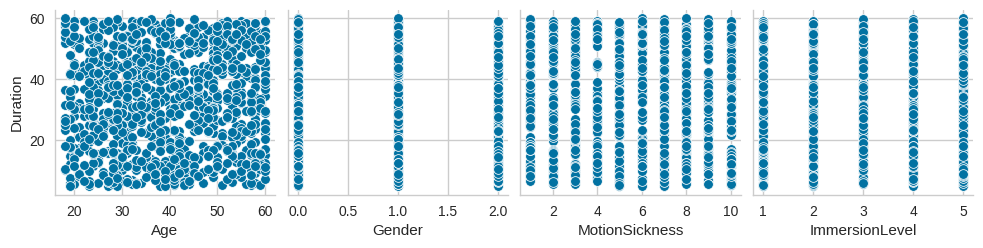
\includegraphics[width=\textwidth]{image.png}
    \caption{caption}
    \label{fig:reference}
\end{figure}

SIDE IMAGES EXAMPLE
\begin{figure}[H]
    \centering
    \begin{subfigure}[b]{0.49\textwidth}
        \centering
        \includegraphics[width=\textwidth]{image1.png}
        \caption{caption1}
        \label{fig:reference1}
    \end{subfigure}
    \hfill
    \begin{subfigure}[b]{0.49\textwidth}
        \centering
        \includegraphics[width=\textwidth]{image2.png}
        \caption{caption2}
        \label{fig:reference2}
    \end{subfigure}
    \caption{total-caption}
    \label{fig:total-reference}
\end{figure}

TABLE EXAMPLE
\begin{table}[!htbp]
    \centering
    \captionsetup{justification=centering}
    \begin{tabular}{|p{4.5cm}|p{9.5cm}|}
        \hline
        a1 & a2\\
        \hline
        b1 & b2 \\
        \hline
    \end{tabular}
    \caption{caption}
    \label{tab:reference}
\end{table}